\documentclass[slidestop,compress,mathserif]{beamer}
%\documentclass[slidestop,compress,mathserif,handout]{beamer}

%\documentclass[xcolor=dvipsnames,handout]{beamer}
%\documentclass[xcolor=dvipsnames]{beamer}

%\documentclass[handout]{beamer}

%%% To get rid of solutions on handouts:
\newcommand{\soln}[1]{\textit{\textcolor{darkGray}{#1}}}				% For slides
%\newcommand{\soln}[1]{ }	% For handouts

% to get pausing to work properly on slides
\newcommand{\hide}[1]{#1}	% For slides
%\newcommand{\hide}[1]{ }	% For handouts
\usepackage{tikz}


%\usepackage{multicol}
\usepackage{amsfonts}
%\usepackage[pdftex,dvipsnames]{color}
\usepackage{graphicx}
\usepackage{subfigure}
%\usepackage{picinpar}
\usepackage{pifont}
\usepackage{pgf,pgfarrows,pgfnodes}
%\usepackage{wasysym,manfnt,phaistos,empheq}
\usepackage[english]{babel}
\usepackage{pgfpages}
\usepackage{natbib}
\usepackage{hyperref}
\usepackage{multimedia}
%\usepackage{amsfonts,amstext,amssymb,amsbsy,amsopn,amsthm,eucal,latexsym,mathrsfs}
\usepackage{amsmath,amsfonts,amstext,amssymb,amsbsy,amsopn,amsthm,eucal,latexsym,mathrsfs}
\usepackage{ulem}
\usepackage{setspace}
\usepackage{array}
%\usepackage{rotating}
\usepackage{multirow}
\usepackage{verbatim}
\usepackage{multicol}

\setbeamertemplate{navigation symbols}{}

%\usepackage{tikz}
%\usetikzlibrary{arrows,shapes,trees,backgrounds}


%\setbeameroption{show notes on second screen}
%\setbeameroption{show notes}
%\setbeameroption{show only notes}

\definecolor{links}{HTML}{2A1B81}
\hypersetup{colorlinks,linkcolor=,urlcolor=links}

\newtheorem*{principle}{Inscrutibility Principle}
\newtheorem*{punchline}{Punch Line}
\newtheorem{defn}{Definition}

\definecolor{Scarlet}{RGB}{140,17,17}
\definecolor{VassarRed}{RGB}{128,0,0}

% "dinglist" environment
  \renewenvironment{dinglist}[2][blue]
  {\begin{list}{\textcolor{blue}{\ding{#2}}}{}}{\end{list}}
  % Symbol definitions for these lists
  \newcommand{\DingListSymbolA}{43}
  \newcommand{\DingListSymbolB}{243}
  \newcommand{\DingListSymbolC}{224}
  \newcommand{\DingListSymbolD}{219}
  \newcommand{\DingListSymbolCheck}{52}
  \newcommand{\DingListSymbolCross}{56}


  \newenvironment{ballotenv}
{\only{%
\setbeamertemplate{itemize item}{\ding{45}}%
\setbeamertemplate{itemize subitem}{\ding{46}}%
\setbeamertemplate{itemize subsubitem}{\ding{46}}}} {}
\setbeamertemplate{itemize item}{\ding{49}}
\setbeamertemplate{itemize subitem}{\ding{47}}
\setbeamertemplate{itemize subsubitem}{\ding{47}}


%User defined colors: See colors section
\xdefinecolor{oiBlue}{rgb}{0.15, 0.35, 0.55}
\xdefinecolor{gray}{rgb}{0.5, 0.5, 0.5}
\xdefinecolor{darkGray}{rgb}{0.3, 0.3, 0.3}
\xdefinecolor{darkerGray}{rgb}{0.2, 0.2, 0.2}
\xdefinecolor{rubineRed}{rgb}{0.89,0,0.30}
\xdefinecolor{linkCol}{rgb}{0.11,0.49,0.95}	
\xdefinecolor{irishGreen}{rgb}{0,0.60,0}	
\xdefinecolor{darkturquoise}{rgb}{0.44, 0.58, 0.86}
\definecolor{lightGreen}{rgb}{0.533,0.765,0.42}
\xdefinecolor{Regalia}{HTML}{522D80}
\xdefinecolor{ClemsonOrange}{HTML}{EA6A20}

\definecolor{duke@LightGrey}{RGB}{200,200,200}\definecolor{DarkGreen}{RGB}{0,100,0}
\definecolor{Oranges}{RGB}{255,127,0}
\definecolor{LightGray}{RGB}{211,211,211}

%\setbeamertemplate{footline}{%
%  \raisebox{5pt}{\makebox[\paperwidth]{\hfill\makebox[10pt]{\scriptsize\insertframenumber}}}}

\setbeamercolor{equation background}{fg=black,bg=duke@LightGrey}
  % Boxed equation
  \newcommand{\eqbox}[2][0.6]{%
  \centerline{
  \begin{beamerboxesrounded}[lower=equation background,width=#1\hsize,shadow=true]{}
\parbox{#1\hsize}{%
      \[
        \textcolor{black} {#2}
      \]}
  \end{beamerboxesrounded}
}}

\AtBeginSection[] {
  \begin{frame}<beamer>\frametitle{Outline}
    \tableofcontents[currentsection,hideothersubsections]
  \end{frame}
}
%
%
%\AtBeginSubsection[] {
%  \begin{frame}<beamer>\frametitle{Outline}
%    \tableofcontents%[currentsection,currentsubsection]
%  \end{frame}
%}

%\usecolortheme[RGB={82,45,128}]{structure}
%\usecolortheme[RGB={162,80,22}]{structure}
\usecolortheme[RGB={128,0,0}]{structure}
\usetheme[secheader]{Boadilla}
%\usetheme[height=7mm]{Rochester}
%\usetheme{Copenhagen}
%\usetheme{Antibes}
%\usecolortheme{seahorse}
%\usecolortheme{crane}
%\usecolortheme{rose}
%\usefonttheme[onlylarge]{structurebold}
%\usefonttheme[onlymath]{serif}



\def\diag{{\rm diag}}


\def\E{\mathbb{E}}
\def\Prob{\mathbb{P}}
\def\argmin{{\rm argmin}}
\def\argmax{{\rm argmax}}
\def\Def{\stackrel{def}{=}}


\newtheorem{assumption}{Assumptions}
\newtheorem*{proposition}{Proposition}
\newtheorem*{remark}{Remark}



%\setbeamercolor{disc title}{bg=oiBlue!40!white!60,fg=blue}
\setbeamercolor{disc body}{bg= Regalia!20!white!80,fg= Regalia!80!black!90}

\setbeamercolor{clicker ungraded title}{bg=irishGreen!80!white!50,fg=irishGreen!30!black!90}
\setbeamercolor{clicker ungraded body}{bg=irishGreen!20!white!80,fg=irishGreen!30!black!90}

\setbeamercolor{clicker review title}{bg=gray!80!white!80,fg=oiBlue!80!black!90}
\setbeamercolor{clicker review body}{bg=gray!30!white!90,fg=oiBlue!80!black!90}

\setbeamercolor{code body}{bg=gray!20!white!80,fg=black}


% Custom commands
\newcommand{\degree}{\ensuremath{^\circ}}
\newcommand{\Note}[1]{
\rule{2.5cm}{0.25pt} \\ \textit{\scriptsize {\textcolor{rubineRed}{Note:} \textcolor{gray}{#1}}}}
\newcommand{\ct}[1]{
\vfill
{\tiny #1}}
\newcommand{\Remember}[1]{\textit{\scriptsize{\textcolor{orange}{Remember:} \textcolor{gray}{#1}}}}
\newcommand{\red}[1]{\textit{\textcolor{rubineRed}{#1}}}
\newcommand{\pink}[1]{\textit{\textcolor{rubineRed!90!white!50}{#1}}}
\newcommand{\green}[1]{\textit{\textcolor{irishGreen}{#1}}}
\newcommand{\webURL}[1]{\urlstyle{same}\textit{\textcolor{linkCol}{\url{#1}}} }
\newcommand{\webLink}[2]{\href{#1}{\textcolor{linkCol}{{#2}}}}
\newcommand{\mail}[1]{\href{mailto:#1}{\textit{\textcolor{linkCol}{#1}}}}
\newcommand{\hl}[1]{\textit{\textcolor{oiBlue}{#1}}}
\newcommand{\hlGr}[1]{\textit{\textcolor{lightGreen}{#1}}}
\newcommand{\mathhl}[1]{\textcolor{oiBlue}{\ensuremath{#1}}}
\newcommand{\ex}[1]{\textcolor{blue}{{{\small (#1)}}}}
\newcommand{\disc}[1]{
\begin{beamerboxesrounded}[shadow = true, lower = disc body, upper = disc title]{}
#1
\end{beamerboxesrounded}
}

\newcommand{\cl}[1]{
\begin{beamerboxesrounded}[shadow = true, lower = clicker ungraded body, upper = clicker ungraded title]{Question}
$\:$ \\
#1
\end{beamerboxesrounded}
}

\newcommand{\clR}[1]{
\begin{beamerboxesrounded}[shadow = true, lower = clicker review body, upper = clicker review title]{\red{Review question} }
$\:$ \\
#1
\end{beamerboxesrounded}
}

\newcommand{\formula}[2]{
\begin{beamerboxesrounded}[shadow = true, lower = white, upper = clicker review body]{#1}
#2
\end{beamerboxesrounded}
$\:$ \\
}

\newenvironment{twocol}[4]{
\begin{columns}[c]
\column{#1\textwidth}
#3
\column{#2\textwidth}
#4
\end{columns}
}


\newenvironment{slot}[2]{
\begin{array}{c}
\underline{#1} \\
#2
\end{array}
}

\newcommand{\pr}[1]{
\left( #1 \right)
}

\newcommand{\solnMult}[1]{
\item[] \vspace{-0.59cm}
\only<beamer| beamer:1>{\item #1}
\soln{\only<2->{\item \red{#1}}}
}

%\newcommand{\codechunk}[1]{
%\begin{beamerboxesrounded}[shadow = true, lower = code body]{}
%{\small #1}
%\end{beamerboxesrounded}
%}

% Change margin

\newenvironment{changemargin}[2]{%
\begin{list}{}{%
\setlength{\topsep}{0pt}%
\setlength{\leftmargin}{#1}%
\setlength{\rightmargin}{#2}%
\setlength{\listparindent}{\parindent}%
\setlength{\itemindent}{\parindent}%
\setlength{\parsep}{\parskip}%
}%
\item[]}{\end{list}}

% Footnote

\long\def\symbolfootnote[#1]#2{\begingroup%
\def\thefootnote{\fnsymbol{footnote}}\footnote[#1]{#2}\endgroup}

% Commands from the book
\newenvironment{data}[1]{\texttt{#1}}{}
\newenvironment{var}[1]{\texttt{#1}}{}
\newenvironment{resp}[1]{\texttt{#1}}{}






%%%%%%%%%%%%%%%%%%%%%%%%%%%%%%%%%%%%%%%%%%%%%%%%%%%%%%%%%%%%%%%%%%%%%%%%%%%%%%%%%%%%%%%%%%%%%%%

\title[Chapter 7 part 1]{Chapter 7 part 1}
\subtitle{Properties of Expectations}

%%%%%%%%%%%%%%%%%%%%%%%%%%%%%%%%%%%%%%%%%%%%%%%%%%%%%%%%%%%%%%%%%%%%%%%%%%%%%%%%%%%%%%%%%%%%%%%


\author[Jingchen (Monika) Hu] % (optional, use only with lots of authors)
{Jingchen (Monika) Hu}
% - Give the names in the same order as the appear in the paper.
% - Use the \inst{?} command only if the authors have different
%   affiliation.

\institute[Vassar] % (optional, but mostly needed)
{Vassar College}
% - Use the \inst command only if there are several affiliations.
% - Keep it simple, no one is interested in your street address.

\date[MATH 241] % (optional, should be abbreviation of conference name)
{MATH 241}
% - Either use conference name or its abbreviation.
% - Not really informative to the audience, more for people (including
%   yourself) who are reading the slides online

\subject{MATH 241}
% This is only inserted into the PDF information catalog. Can be left
% out.



% If you wish to uncover everything in a step-wise fashion, uncomment
% the following command:

%\beamerdefaultoverlayspecification{<+->}


\begin{document}

%\begin{frame}%[plain]
%
\includegraphics[width = \textwidth]{figures/2015DukeNCAA}
%\end{frame}

%{ % all template changes are local to this group.
%\addtocounter{framenumber}{-1}
%    \setbeamertemplate{navigation symbols}{}
%    \begin{frame}[plain]
%        \begin{tikzpicture}[remember picture,overlay]
%            \node[at=(current page.center)] {
%                
\includegraphics[width=1.25\paperwidth]{figures/2015DukeNCAA}
%            };
%        \end{tikzpicture}
%     \end{frame}
%}

%%%%%%%%%%%%%%%%%%%%%

% Title Page

\begin{frame}%[plain]
\titlepage
\end{frame}


%%%%%%%%%%%%%%%%%%%%%%
%\addtocounter{framenumber}{-1}
%
%\begin{frame}\frametitle{Annoucement}
%
%\begin{itemize}
%%\item HW7: \red{due now!}
%\item HW8: \red{due Tuesday, Nov 20th}
%
%
%\vspace{0.5cm}
%\item Course evaluation open tomorrow.
%  \begin{itemize}
%  \item Activate between 11/14 - 12/3.
%  \item If response rate $\geq 80\%$, drop the lowest quiz.
%  \end{itemize}
%
%\vspace{0.5cm}
%\item Next quiz: Tuesday, Nov 18th\\
%  \begin{itemize}
%  \item Topic: function of a continuous random variable, i.e., find $f_Y(y)$ where $Y = g(X)$.
%  %\item To prepare: do homework questions in Chapter 5: 37, 39, 40, TE29
%  \end{itemize}
%
%
%%\item Midterm: Tuesday, Feb 25th
%%\begin{itemize}
%%\item Close book, in class exam (75 min)
%%\item ONE page cheat sheet {\bf made by yourself} (A4 size)
%%\item Calculators are allowed, but not cell phones, tablets or laptops
%%\end{itemize}
%
%\end{itemize}
%
%
%\end{frame}
%

%
%%%%%%%%%%%%%%%%%%%%%%
%\begin{frame}{Outline}
%%\tableofcontents[hideallsubsections,pausections]
%\tableofcontents[hideallsubsections]
%\end{frame}

%%%%%%%%%%%%%%%%%%%%%%%%%%%%%%%%%%%%%%%%%%%
%\begin{frame}\frametitle{Recap}
%
%
%\end{frame}





%%%%%%%%%%%%%%%%%%%%%
%\begin{frame}{Outline}
%%\tableofcontents[hideallsubsections,pausections]
%\tableofcontents[hideallsubsections]
%\end{frame}



%%%%%%%%%%%%%%%%%%%%%%%%%%%%%%%%%%%%%%%%%%
\section{Expectation of sums of random variable}
%%%%%%%%%%%%%%%%%%%%%%%%%%%%%%%%%%%%%%%%%%
\begin{frame}
\frametitle{Expected value of $g(X, Y)$}
Recap: expectation of random variable $g(X)$
\begin{itemize}
\item Discrete case $E[g(X)] = \sum_{\text{all } x} g(x) f(x)$
\item Continuous case $E[g(X)] = \int_{-\infty}^{\infty} g(x)f(x) dx$
\end{itemize}
\pause

Suppose $g(X,Y)$ is a real-valued function of random variables $X$ and $Y$, then

\begin{itemize}
\item Discrete case
\[E[g(X, Y)] = \sum_{\text{all } x}~\sum_{\text{all } y} g(x,y) f(x, y)\]
\item Continuous case
\[E[g(X, Y)] = \int_{-\infty}^{\infty}\int_{-\infty}^{\infty} g(x,y) f(x, y)dxdy\]
\end{itemize}


\end{frame}

%%%%%%%%%%%%%%%%%%%%%%%%%%%%%%%%%%%%%%%%%%

\begin{frame}
%\frametitle{Constrained Sum of Poissons}

\disc{Example: let $X$ and $Y$ be random variables with joint pdf $f(x, y)$. Find $E(X + Y)$}

%\invisible{
\pause

\begin{align*}
E(X + Y) &= \int_{-\infty}^{\infty}\int_{-\infty}^{\infty} (x+y) f(x, y)~dx~dy \\
\uncover<3->{
             &=\int_{-\infty}^{\infty}\int_{-\infty}^{\infty} x f(x, y){\color{red} ~dy~dx} } \uncover<4->{+ \int_{-\infty}^{\infty}\int_{-\infty}^{\infty} y f(x, y)~dx~dy \\}
\uncover<5->{
             &=\int_{-\infty}^{\infty} x \left[\int_{-\infty}^{\infty}  f(x, y)dy \right]dx }
             \uncover<6->{+ \int_{-\infty}^{\infty}y \left[\int_{-\infty}^{\infty}  f(x, y)dx \right] dy \\}
\uncover<7->{
             & = \int_{-\infty}^{\infty} x f_X(x) dx  + \int_{-\infty}^{\infty}y  f_Y(y) dy\\ }
\uncover<8->{
             & = E(X)  + E(Y) }
\end{align*}
%}

\end{frame}

%%%%%%%%%%%%%%%%%%%%%%%%%%%%%%%%%%%%%%%%%%

\begin{frame}\frametitle{Expectation of sums of two random variables}

\[ E(X + Y) = E(X) + E(Y) \]

\pause
\begin{itemize}
\item It's not difficult to show that if either (or both) of the $X, Y$ is discrete, this formula still holds. \pause
\item This results does not require $X$ and $Y$ to be independent. \pause
\item This can be generalized to $n$ random variables
\[E(X_1 + X_2 + \cdots + X_n) = E(X_1) + E(X_2) + \cdots + E(X_n)\] \pause
%}
\item How about $E(XY)?$
\end{itemize}

\end{frame}

%%%%%%%%%%%%%%%%%%%%%%%%%%%%%%%%%%%%%%%%%%
\begin{frame}
\disc{Let $X$ and $Y$ be INDEPENDENT random variables with joint pdf $f(x, y)$. Find $E(XY)$.}

%\invisible{
\pause

\begin{align*}
E(XY) &= \int_{-\infty}^{\infty}\int_{-\infty}^{\infty} xy f(x, y)~dx~dy \\
\uncover<3->{
             &= \int_{-\infty}^{\infty}\int_{-\infty}^{\infty} xy f_X(x) f_Y(y)~dx~dy \\}
\uncover<4->{
             &= \int_{-\infty}^{\infty}y f_Y(y)\left[\int_{-\infty}^{\infty} x f_X(x)dx \right] dy \\}
\uncover<5->{
             & = E(X) \int_{-\infty}^{\infty}y f_Y(y)  dy \\ }
\uncover<6->{
             & = E(X)E(Y) }
\end{align*}
\vfill
\uncover<7->{
Note: (1) this formula only holds when $X$ and $Y$ are independent.\\
(2) This is not a sufficient condition for independence.
}
%}
\end{frame}


%%%%%%%%%%%%%%%%%%%%%%%%%%%%%%%%%%%%%%%%%%
\begin{frame}\frametitle{Recap}

Expectation of sum
\[E[X_1 + X_2 + \cdots + X_n] = E[X_1] + E[X_2] + \cdots + E[X_n]\]
\pause

$X_1, X_2, \ldots, X_n$ are independent $\Longrightarrow$ \red{$\not\Longleftarrow$}
\[E[X_1  X_2  \cdots  X_n] = E[X_1]  E[X_2]  \cdots  E[X_n]\]

\end{frame}

%%%%%%%%%%%%%%%%%%%%%%%%%%%%%%%%%%%%%
%\begin{frame}\frametitle{Distribution of a function of a discrete random variable}
%
%\cl{1. Let $X$ have a Bin$(n, p)$ distribution. What's the pmf of $Y = 2X$?}
%
%\begin{enumerate}[(a)]
%\item $f_Y(y) = {2n \choose y}(2p)^y (1-2p)^{2n - y}$ for any $y \in \{0, 2, 4, \ldots, 2n\}$
%\item $f_Y(y) = {2n \choose y}p^y (1-p)^{2n - y}$ for any $y \in \{0, 1, 2, \ldots, 2n\}$
%\solnMult{$f_Y(y) = {n \choose y/2}p^{\frac{y}{2}} (1-p)^{n - \frac{y}{2}}$ for any $y \in \{0, 2, 4, \ldots, 2n\}$}
%\item $f_Y(y) = \frac{1}{2}{n \choose y/2}p^{\frac{y}{2}} (1-p)^{n - \frac{y}{2}}$ for any $y \in \{0, 2, 4, \ldots, 2n\}$
%\end{enumerate}
%
%%\invisible{
%\pause
%\[ f_Y(y) = P(Y = y) = P\left(X = \frac{y}{2}\right) = f_X\left(\frac{y}{2}\right) \]
%
%%}
%
%\end{frame}
%


%%%%%%%%%%%%%%%%%%%%%%
%\begin{frame}{Outline}
%%\tableofcontents[hideallsubsections,pausections]
%\tableofcontents[hideallsubsections]
%\end{frame}



%%%%%%%%%%%%%%%%%%%%%%%%%%%%%%%%%%%%%%%%%%
\section{Covariance and correlation}
%%%%%%%%%%%%%%%%%%%%%%%%%%%%%%%%%%%%%%%%%%

\begin{frame}\frametitle{Covariance}
\begin{defn}
\hl{Covariance} of two random variables $X$ and $Y$ is defined as
\[ Cov(X,Y) = E[ (X-E[X]) (Y-E[Y]) ] \]
\end{defn}
\pause
\begin{itemize}
\item Simplification
\begin{align*}
    Cov(X,Y)  &= E[ (X-\mu_X) (Y-\mu_Y) ]\\
             &= E[ XY+\mu_X\mu_Y-X\mu_Y-Y\mu_X]) \\
             &= E[XY]-\mu_X\mu_Y \\
\end{align*}
\pause \vspace{-0.7cm}
\item Recall
\begin{align*}
    E[XY]  &= \int\int xy ~f(x, y) ~dx~dy ~~ \text{ if continuous }\\
             &= \sum_x \sum_y xy~ f(x, y)~~ \text{ if discrete }
\end{align*}
\end{itemize}

\end{frame}

%%%%%%%%%%%%%%%%%%%%%%%%%%%%%%%%%%%%%%%%%%

\begin{frame}\frametitle{Properties of $Cov(X,Y) = E[XY]- E[X]E[Y]$}
\begin{itemize}
\item $Cov(X,Y) = Cov(Y, X)$
\pause
\item $Cov(X,c) = 0$
\pause
\item $Cov(X,X) = Var(X)$
\pause
\item $Cov(aX,bY) = \uncover<4->{ab~Cov(X,Y)}$
\pause
%\invisible{
\uncover<4->{
\begin{align*}
Cov(aX,bY) & = E[abXY] - E[aX]E[bY] \\
	& = ab~E[XY] - ab~E[X]E[Y]
\end{align*}
%}
}
\pause
\vspace{-0.5cm}
\item \uncover<5->{
$Cov(X+a,Y+b) = \uncover<5->{Cov(X,Y)}$}
%\invisible{
\pause
\uncover<5->{
\begin{align*}
Cov(X + a,Y+b) = & E[(X+a)(Y+b)] - E[X+a]E[Y+b] \\
	= & ~E[XY + aY + bX + ab] \\
	& - (E[X] + a) (E(Y)+b)\\
	= & ~E[XY] + E[aY] + E[bX] + ab \\
	& - E[X]E[Y] - a~E[Y] -b~E[X] - ab \\
	= & ~E[XY]- E[X]E[Y]
\end{align*}
%}
}
\end{itemize}

\end{frame}

%%%%%%%%%%%%%%%%%%%%%%%%%%%%%%%%%%%%%%%%%%
\begin{frame}\frametitle{Covariance of sums of random variables}
\[Cov\left(\sum_{i=1}^n X_i, \sum_{j = 1}^m Y_j  \right) = \sum_{i=1}^n \sum_{j = 1}^m Cov\left(X_i, Y_j  \right)\]
\pause
A special case
\[Var\left(\sum_{i=1}^n X_i \right) = \sum_{i=1}^n Var(X_i) + 2\sum_{1 \leq i < j \leq n} Cov(X_i, X_j)\]
\pause
Some more special cases
\begin{align*}
Var(X+Y) &= Var(X)+Var(Y)+2Cov(X,Y)\\
Var(X-Y) &= Var(X)+Var(Y)-2Cov(X,Y)\\
\end{align*}


\end{frame}

%%%%%%%%%%%%%%%%%%%%%%%%%%%%%%%%%%%%%%%%%%

\begin{frame}\frametitle{Zero covariance and independence}

\begin{itemize}
\item $X$ and $Y$ are independent $ \Longrightarrow$ $Cov(X,Y) = 0$
\pause
\[ Cov(X,Y) = E[XY]- E[X]E[Y] = E[X]E[Y] - E[X]E[Y] = 0\] \pause
\item $X_1, X_2, \ldots, X_n$ are independent $ \Longrightarrow$
\[Var\left(\sum_{i=1}^n X_i \right) = \sum_{i=1}^n Var(X_i)\]
\pause
\item $Cov(X,Y) = 0 \not\Longrightarrow$  $X$ and $Y$ are independent\\
Counter example?

\end{itemize}

\end{frame}

%%%%%%%%%%%%%%%%%%%%%%%%%%%%%%%%%%%%%%%%%%
\begin{frame}\frametitle{Counter example}
\disc{Let $X \sim \text{Unif}(-0.5, 0.5)$ and $Y = X^2$.
Find $Cov(X, Y)$, and decide if $X$ and $Y$ and independent.
}
\pause
Covariance \pause
\[E[X] = 0, ~ E[XY] = E[X^3] = \int_{-0.5}^{0.5} x^3 dx = \left. \frac{x^4}{4} \right|_{-0.5}^{0.5} = 0\] \pause
\[Cov(X, Y) = E[XY] - E[X] E[Y] = E[X^3] - E[X] E[X^2] = 0 \] \pause
Independence: \pause
since $Y$ depends on $X$, so not independent. \\ \pause
(To be more rigorous, we need to show \[f(x, y) \neq f_X(x)f_Y(y)\] for some $x, y \in \mathbb{R}$.)


\end{frame}

%%%%%%%%%%%%%%%%%%%%%%%%%%%%%%%%%%%%%%%%%%
\begin{frame}
\frametitle{Correlation}

Since $Cov(X,Y)$ depends on the magnitude of $X$ and $Y$ we would prefer to have a measure of association that is not effected by arbitrary changes in the scales of the random variables.\\

\begin{defn}
The most common measure of \emph{linear} association is \hl{correlation} which is defined as
\[ \rho(X,Y) = \frac{Cov(X,Y)}{\sqrt{Var(X)}~\sqrt{Var(Y)}}  \]
\end{defn}
\pause
\begin{itemize}
\item range: $-1 \leq \rho(X,Y) \leq 1 $
\item the magnitude (i.e.\ absolute value) of the $\rho(X,Y)$ measures the strength of the \emph{linear} association
\item the sign determines if it is a positive or negative relationship.
\item if $\rho(X, Y) = 0$, then $X$ and $Y$ are said to be uncorrelated.
\end{itemize}
\end{frame}



%%%%%%%%%%%%%%%%%%%%%%%%%%%%%%%%%%%%%%%%%%

\begin{frame}
\frametitle{Correlation}

\vfill

\begin{center}
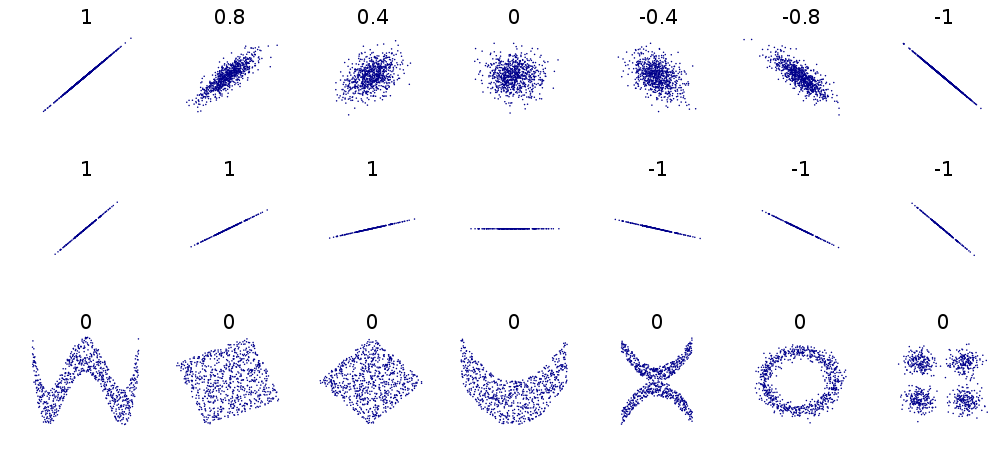
\includegraphics[width=\textwidth]{figures/corr.png}
\end{center}

\vfill

\end{frame}


%%%%%%%%%%%%%%%%%%%%%%%%%%%%%%%%%%%%%%%%%%
\section{Conditional expectation}
%%%%%%%%%%%%%%%%%%%%%%%%%%%%%%%%%%%%%%%%%%
\begin{frame}\frametitle{Conditional expectation}
\begin{itemize}
\item The discrete case: for all $p_Y(y) > 0$
\begin{itemize}
\item Conditional pmf: $p_{X \mid Y}(x \mid y) = P\{X = x \mid  Y = y\} = \frac{p(x, y)}{p_Y(y)}$
{\small{
\begin{block}{Definition}
The conditional expectation of $X$ given that $Y = y$ is
$$E[X \mid Y = y] = \sum_x xP\{X = x \mid  Y = y\} = \sum_x xp_{X \mid Y}(x \mid y)$$
\end{block}
}}
\end{itemize}
\pause
\item The continuous case: for all $f_Y(y) > 0$
\begin{itemize}
\item Conditional pdf: $f_{X \mid Y}(x \mid y) = \frac{f(x, y)}{f_Y(y)}$
{\small{
\begin{block}{Definition}
The conditional expectation of $X$ given that $Y = y$ is
$$E[X \mid Y = y] = \int_{-\infty}^{\infty}xf_{X \mid Y}(x \mid y)dx$$
\end{block}
}}
\end{itemize}
\end{itemize}
\end{frame}

\begin{frame}\frametitle{Properties of expectations remain}
\begin{itemize}
\item Expectation of a function of a random variable
\begin{itemize}
\item The discrete case:
$$E[g(X) \mid Y = y] = \sum_x g(x)p_{X \mid Y}(x \mid y)$$
\item The continuous case:
$$E[g(X) \mid Y = y] = \int_{-\infty}^{\infty}g(x)f_{X \mid Y}(x \mid y)dx$$
\end{itemize}
\pause
\vspace{2mm}
\item Expectation of sum of random variables
$$E[\sum_{i=1}^n X_i \mid Y = y] = \sum_{i=1}^n E[X_i \mid Y = y]$$
\vspace{2mm}
\pause
\item Think about the condition $Y = y$ as taking expectation of $X$ on a reduced sample space consisting only of outcomes for which $Y = y$
\end{itemize}
\end{frame}

\begin{frame}\frametitle{Computing expectations by conditioning}
$$E[X] = E[E[X\mid Y]]$$
\begin{itemize}
\item A very important property of conditional expectation
\item Think of $E[X|Y]$ as a random variable (when $Y = y$)
\item The discrete case:
$$E[X] = \sum_y E[X\mid Y = y]P\{Y = y\}$$
\item Intuition:
\begin{itemize}
\item $E[E[X\mid Y]]$ is a weighted average of $E[X\mid Y]$, where weights are $P\{Y = y\}$ (the probability of the condition)
\item Similar to the ``law of total probability" $P(E) = \sum_{i=1}^n P(E\mid F_i)P(F_i)$
\end{itemize}
\vspace{2mm}
\pause
\item The continuous case:
$$E[X] = \int_{-\infty}^{\infty}E[X\mid Y = y]f_Y(y)dy$$
\end{itemize}
\end{frame}

\begin{frame}
\disc{{\small{A miner is trapped in a mine containing 3 doors. The 1st door leads to a tunnel that will take him to safety after 3 hours of travel. The 2nd door leads to a tunnel that will return him to the mine after 5 hours of travel. The 3rd door leads to a tunnel that will return him to the mine after 7 hours. If we assume that the miner is at all times equally likely to choose any one of the doors, what is the expected length of time until he reaches safety?}}}
\pause
{\small{
\begin{itemize}
\item Let $X$ denote the amount of time in hours until he reaches safety, and $Y$ denote the door he initially chooses.
{\scriptsize{
\begin{eqnarray*}
E[X] &=& E[X \mid Y = 1]P\{Y = 1\} + E[X \mid Y = 2]P\{Y = 2\} + E[X \mid Y = 3]P\{Y = 3\} \\
&=&
 \frac{1}{3}(E[X \mid Y = 1] + E[X \mid Y = 2] + E[X \mid Y = 3])
\end{eqnarray*}
}}
\pause
\item Note that $E[X|Y = 1] = 3, E[X \mid Y = 2] = 5 + E[X], E[X \mid Y = 3] = 7 + E[X]$
\item Therefore $E[X] = \frac{1}{3}(3 + 5 + E[X] + 7 + E[X])$, which gives $E[X] = 15$
\end{itemize}
}}
\end{frame}


\begin{frame}\frametitle{Computing probabilities by conditioning}
\begin{itemize}
\item Let $E$ denote an arbitrary event, and define the indicator random variable $X$ as
\[ X = \begin{cases}
    1& \text{if $E$ occurs } \\
    0         & \text{if $E$ does not occur}
\end{cases}
 \]
\item Then $E[X] = P(E), E[X \mid Y = y] = P(E \mid Y = y)$ for any random variable $Y$
\vspace{2mm}
\item The discrete case:
$$P(E) = \sum_yP(E \mid Y = y)p(Y = y)$$
related to $P(E) = \sum_{i=1}^nP(E \mid F_i)P(F_i)$
\vspace{2mm}
\pause
\item The continuous case:
$$P(E) = \int_{-\infty}^{\infty}P(E \mid Y = y)f_Y(y)dy$$
\end{itemize}
\end{frame}

%\begin{frame}
%\disc{Suppose that $X$ and $Y$ are independent continuous random variables. Find the distribution of $X + Y$.}
%\pause
%By conditioning on the value of $Y$
%\begin{eqnarray*}
%P\{X + Y < z\} &=& \int_{-\infty}^{\infty}P\{X + Y < z| Y = y\}f_Y(y)dy\\
%\pause
%&=&
%\int_{-\infty}^{\infty}P\{X + y < z\}f_Y(y)dy\\
%\pause
%&=&
%\int_{-\infty}^{\infty}P\{X < z - y\}f_Y(y)dy\\
%\pause
%&=&
%\int_{-\infty}^{\infty}F_X(z - y)f_Y(y)dy
%\end{eqnarray*}
%\end{frame}

\begin{frame}\frametitle{Conditional variance}
\begin{itemize}
\item Similarly to the conditional expectation, we can define the conditional variance of $X$ given that $Y = y$
\begin{block}{Definition}
$$Var(X \mid Y = y) = E[(X - E[X \mid Y = y])^2  \mid  Y = y]$$
\end{block}
\pause
\item A very useful conditional variance formula
$$Var(X) = E[Var(X \mid Y)] + Var(E[X \mid Y])$$
\end{itemize}
\end{frame}

\end{document}
